\documentclass[10pt,border=1pt]{standalone}
\usepackage[T1]{fontenc}
\usepackage{mathptmx}
\usepackage{amsmath,amssymb}
\usepackage[table]{xcolor}
\usepackage{tikz}
\usetikzlibrary{positioning,arrows.meta,calc,fit,decorations.pathreplacing}
\definecolor{fmblue}{HTML}{2A78D6}
\definecolor{cnnorange}{HTML}{EB6834}
\definecolor{inkgray}{HTML}{52514E}
\definecolor{lightfill}{HTML}{F1F0EC}
\tikzset{
  arr/.style={-{Stealth[length=2.2mm]}, draw=inkgray, line width=0.7pt},
  blk/.style={draw=inkgray, rounded corners=2pt, fill=white, align=center, inner sep=3pt, font=\fontsize{10}{12}\selectfont},
  frz/.style={blk, fill=lightfill},
  trn/.style={blk, fill=fmblue!14},
  trn2/.style={blk, fill=cnnorange!16},
  note/.style={align=left, font=\fontsize{10}{12}\selectfont\itshape, text=inkgray},
}
\begin{document}
\fontsize{10}{12}\selectfont

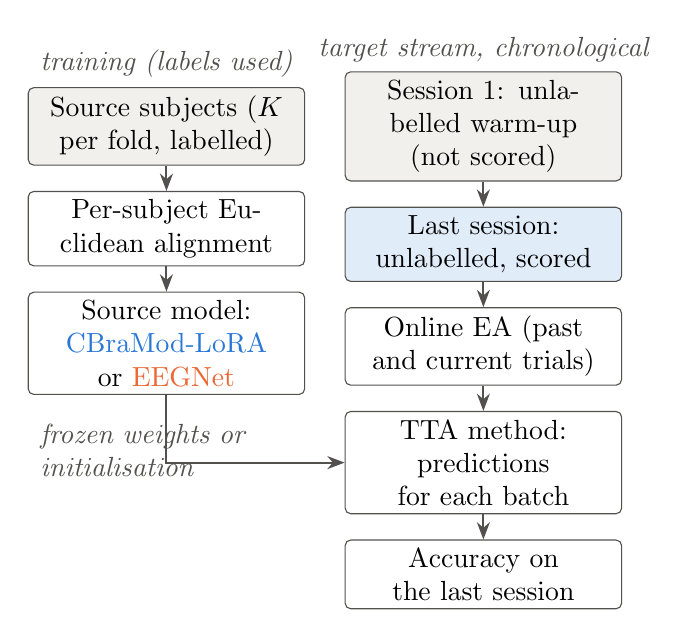
\begin{tikzpicture}[node distance=0.32cm]
\node[frz, text width=3.3cm] (S) {Source subjects ($K$ per fold, labelled)};
\node[blk, text width=3.3cm, below=of S] (EA) {Per-subject Euclidean alignment};
\node[blk, text width=3.3cm, below=of EA] (M) {Source model: {\color{fmblue}CBraMod-LoRA} or {\color{cnnorange}EEGNet}};
\draw[arr] (S)--(EA); \draw[arr] (EA)--(M);
\node[note, anchor=south] at (S.north) {training (labels used)};
\node[frz, text width=3.3cm, right=0.5cm of S] (T1) {Session 1: unlabelled warm-up (not scored)};
\node[trn, text width=3.3cm, below=of T1] (T2) {Last session: unlabelled, scored};
\node[blk, text width=3.3cm, below=of T2] (O) {Online EA (past and current trials)};
\node[blk, text width=3.3cm, below=of O] (A) {TTA method: predictions for each batch};
\node[blk, text width=3.3cm, below=of A] (Y) {Accuracy on the last session};
\draw[arr] (T1)--(T2); \draw[arr] (T2)--(O); \draw[arr] (O)--(A); \draw[arr] (A)--(Y);
\draw[arr] (M.south) |- (A.west);
\node[note, anchor=south] at (T1.north) {target stream, chronological};
\node[note, text width=3.2cm, below=0.25cm of M] {frozen weights or initialisation};
\end{tikzpicture}
\end{document}
